
\begin{figure}[htbp]
\centering
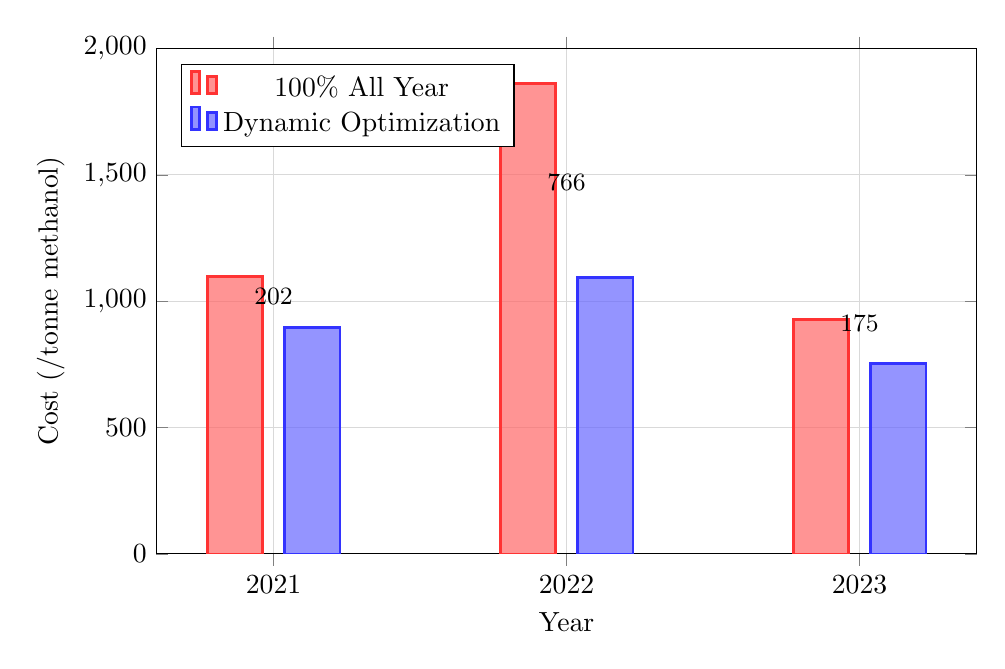
\begin{tikzpicture}
\begin{axis}[
    width=12cm,
    height=8cm,
    xlabel={Year},
    ylabel={Cost (\euro/tonne methanol)},
    ymin=0,
    ymax=2000,
    xtick=data,
    symbolic x coords={2021,2022,2023},
    legend pos=north west,
    grid=major,
    grid style={gray!30},
    bar width=20pt,
    ybar=8pt,
    enlarge x limits=0.2,
    every axis plot/.append style={
        fill opacity=0.7,
        draw opacity=1,
        line width=1pt
    }
]

% 100% All Year Strategy
\addplot[
    fill=red!60,
    draw=red!80,
] coordinates {
    (2021,1099)
    (2022,1860)
    (2023,927)
};

% Dynamic Optimization Strategy
\addplot[
    fill=blue!60,
    draw=blue!80,
] coordinates {
    (2021,897)
    (2022,1094)
    (2023,752)
};

% Add savings annotations
\node at (axis cs:2021,950) [anchor=south] {\small \euro202};
\node at (axis cs:2022,1400) [anchor=south] {\small \euro766};
\node at (axis cs:2023,840) [anchor=south] {\small \euro175};

\legend{100\% All Year, Dynamic Optimization}

\end{axis}
\end{tikzpicture}
\caption{Cost comparison between continuous operation and dynamic optimization strategies across different years}
\label{fig:cost-comparison}
\end{figure}
